\section{A realistic analysis scenario}
\label{sec:validation_realistic}

Everything up to this point has been measured on the generated samples with no selection
applied. An analysis sees instead the events that survive a trigger, a reconstruction and
a set of cuts, in one corner of phase space that the basis optimization knew nothing
about, as raw LHE kinematics was used at that step. This section applies the method in the signal region of $\HH\to\bbbar\bbbar$, using the public
release of Ref.~\cite{CMS:2026znu,hepdata.171917}, and measures the performance of the developed tools in realistic phase spaces.

The release provides generator-level trees with the two Higgs boson four-vectors and the
event weight, for both resolved and a fully merged topologies, at four values of
$\kappa_\lambda$---therefore outside SMEFT parameter space. Since the trees carry \mHH, $\cos\theta^*$ and
$\pt^{\HH}$ event by event, the ELR can use them as an input to the multi-ref approach to produce templates at any point of the SMEFT parameter space, before or after the selection. With this procedure we generate all the BPs after the SR selection.

In order to explore the MM coverage of the full 9D parameter space in the SR, one can investigate the acceptance times efficiency provided by each topology by doing 1D scans for each of the Wilson coefficients, and then comparing the smooth interpolation given by the MM with the outcome obtained with the ELR evaluated in a few points of the scan. Figure~\ref{fig:acc_4b} shows how the selection efficiency varies as a function of each of the relevant Wilson coefficients, hinting which corners of the parameter space are favored according to each topology. This is then summarized on Table \ref{tab:acceptance_response}, which shows how each topology responds to variations in each Wilson coefficient. It can be noticed that the boosted selection zooms in on the coefficients that populate the high-mass tail (e.g., $c_{\text{HG}}$ and $c_{u\text{H}}$), while in the resolved case, a larger portion of the kinematic phase space is selected and the topology averages over different structures, therefore not strongly favoring some coefficients over others. Additionally, the impact of the chromomagnetic operator is similar to that of the leading operators, while the four-fermion operators indeed exhibit subtle changes in the acceptance, with $c^{(1)}_{\text{Qt}}$ and $c^{(8)}_{\text{Qt}}$ being nearly degenerated, and $c^{(8)}_{\text{QQ}}$ the least impactful.

It must be noticed that an operator may change the cross section by a large factor and the acceptance not at all, meaning that the information extracted from Figure \ref{fig:acc_4b} and Table \ref{tab:acceptance_response} must be complemented with a notion about how the overall cross section behaves in the parameter space---It does not really matter if, for instance, the boosted topology has 100\% selection efficiency in a corner of the parameter space where the overall cross section is orders of magnitude smaller than in regions where the same selection has an acceptance times efficiency of 10\%.





%The quantity throughout is the acceptance times efficiency, the template integral over
%the cross section, in which the luminosity and the next-to-next-to-leading-order factor
%cancel. Fig.~\ref{fig:acc_4b} shows it against each Wilson coefficient in turn, the other
%eight held at zero, for both selections.

%The curves of Fig.~\ref{fig:acc_4b} are built from the basis templates, which the
%reweighting itself produced. The reweighting therefore appears on both sides of them and
%the basis points are reproduced by construction, so on their own the curves establish
%that the interpolation is smooth, not that it is right. The test is to apply the
%reweighting directly: the same events are reweighted to a point that is not in the basis,
%the same selection is applied, and the integral is compared with what the matrix method
%predicts there from the forty templates. Fifty-two such points were produced, eight or
%nine along each of the six coefficients of Fig.~\ref{fig:acc_4b} and over the full range
%of each, in both selections: the open circles of that figure. Every one of them agrees
%with the matrix method to better than $0.1\%$. Each point carries the
%statistical error of the reweighted template combined with that of the reweighting
%coefficients, and the error bars are smaller than the markers almost everywhere.

%Those deviations are smaller than the uncertainty of the templates themselves at every
%point, which the same figure shows as bands. The accuracy quoted in
%Sec.~\ref{sec:validation_mm} without a selection therefore survives one, in both
%selections and along every coefficient the selections respond to. Both selections agree
%at a level set by numerical precision rather than by any property of the phase space:
%once the two sides use the same reweighting, the same input treatment and the same
%binning, the matrix method reproduces the reweighting. This is a statement that the
%morphing is algebraically faithful to the parameterization it is built on, not that
%either description of the high-mass tail has been verified against simulation there. The
%only point in this section that tests more than that is the SM, where a directly
%generated sample exists and is compared with the reweighted prediction; the closure of
%the methods against samples they were not built from is the subject of
%Sec.~\ref{sec:validation_mm}.

%Comparing the matrix method against the reweighting over a plane would need the
%reweighting evaluated directly on a grid of points rather than along a line, which is a
%large amount of computation for a figure whose conclusion a one-dimensional scan already
%carries. The verification here is therefore one-dimensional throughout. The planes that
%do appear below ask which operators matter in a selected phase space rather than whether
%the interpolation is faithful, and they cost only evaluations of the model.

\begin{figure}[htbp]
    \centering
    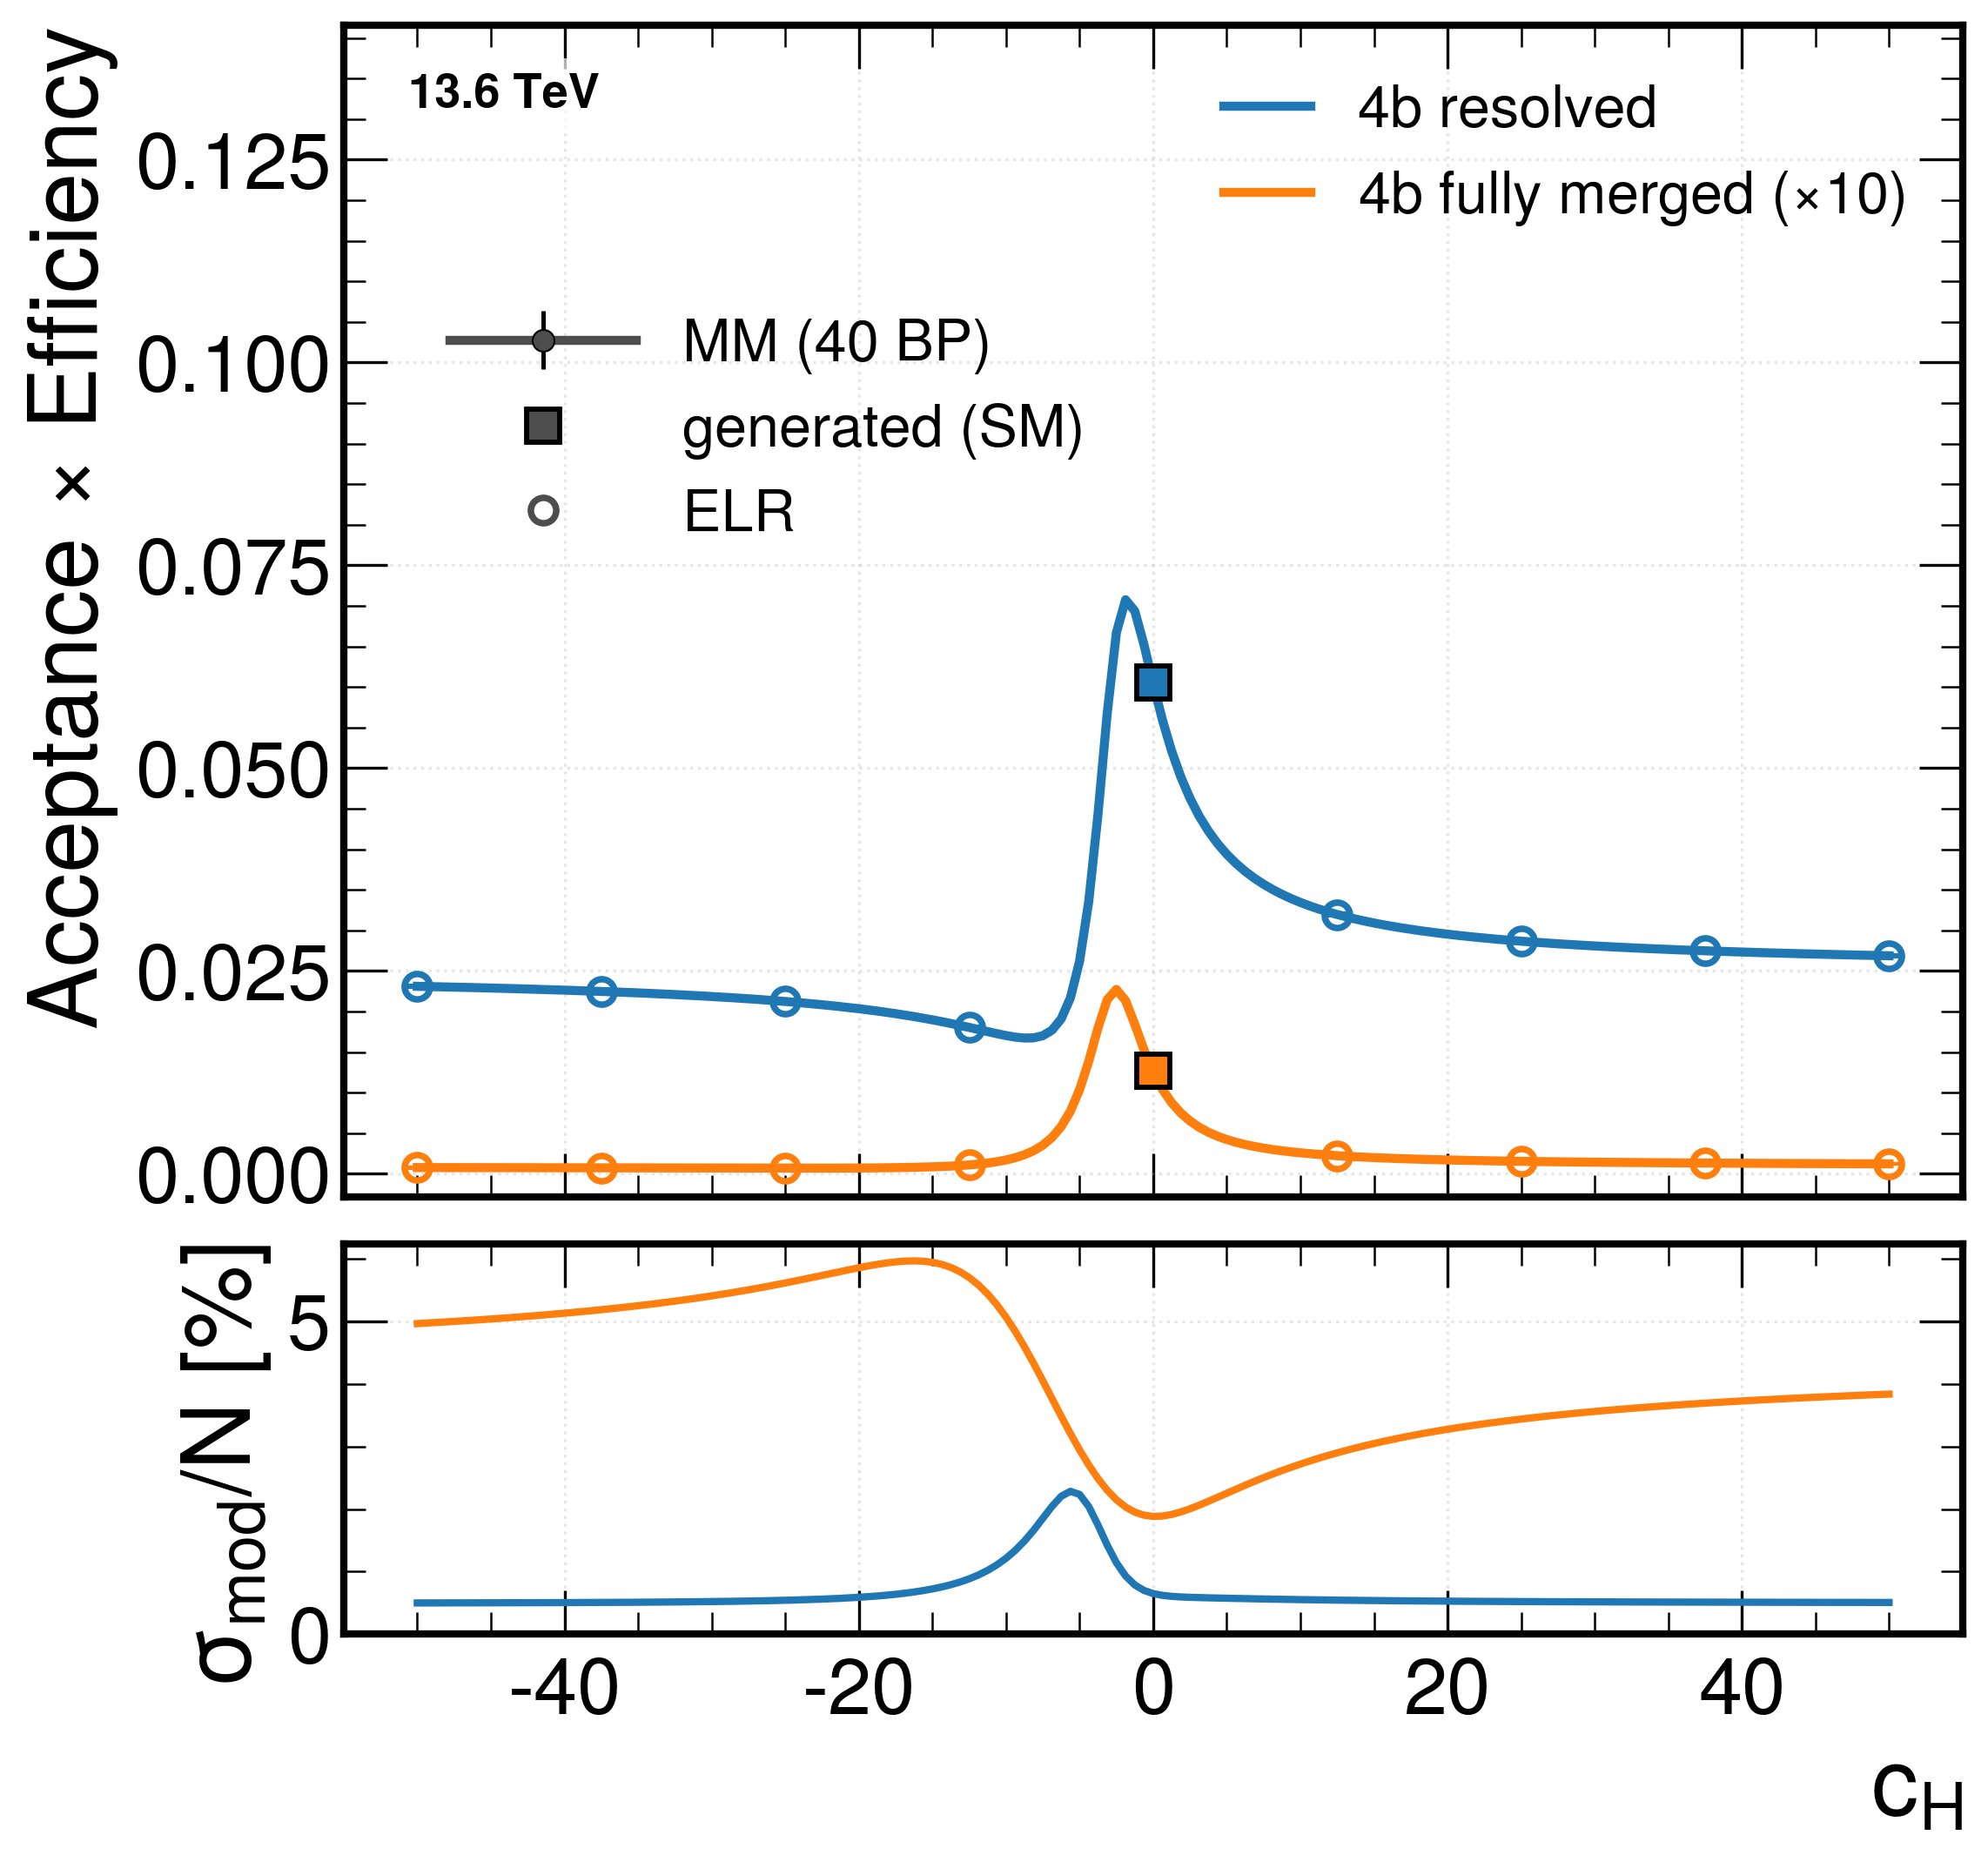
\includegraphics[width=0.32\textwidth]{figures/basis_optimization/eff4b_cH.png}
    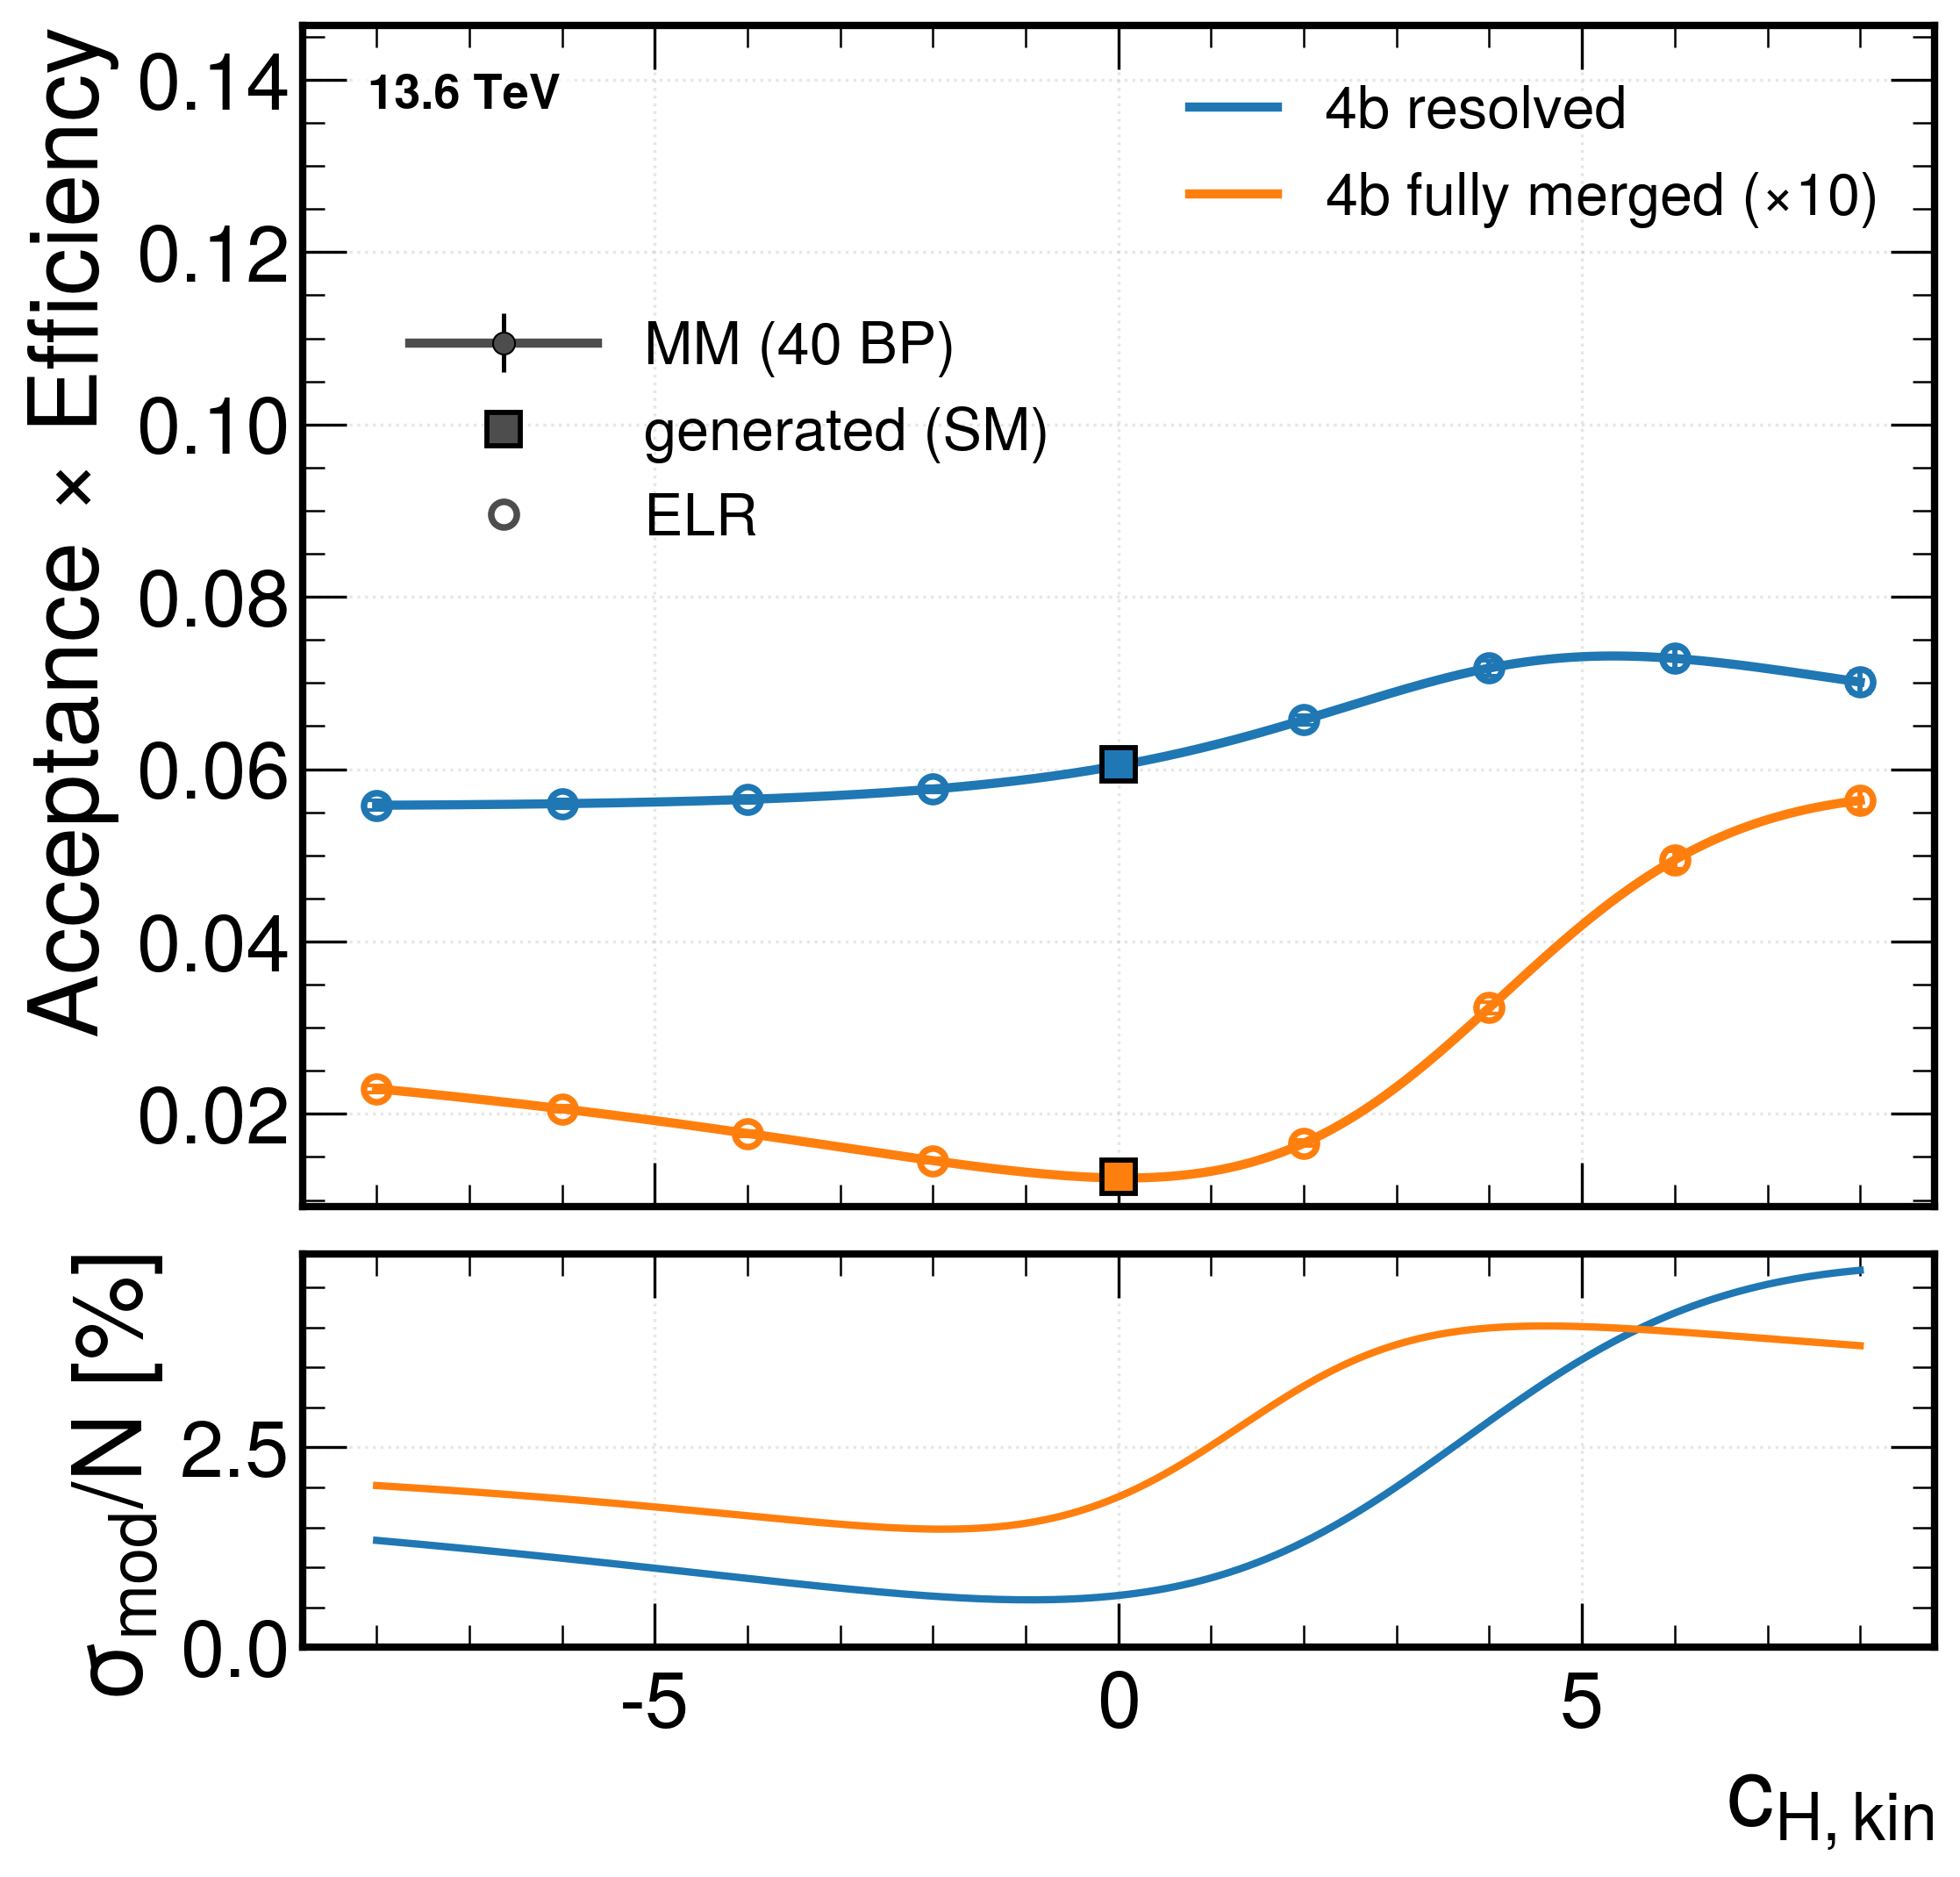
\includegraphics[width=0.32\textwidth]{figures/basis_optimization/eff4b_cHkin.png}
    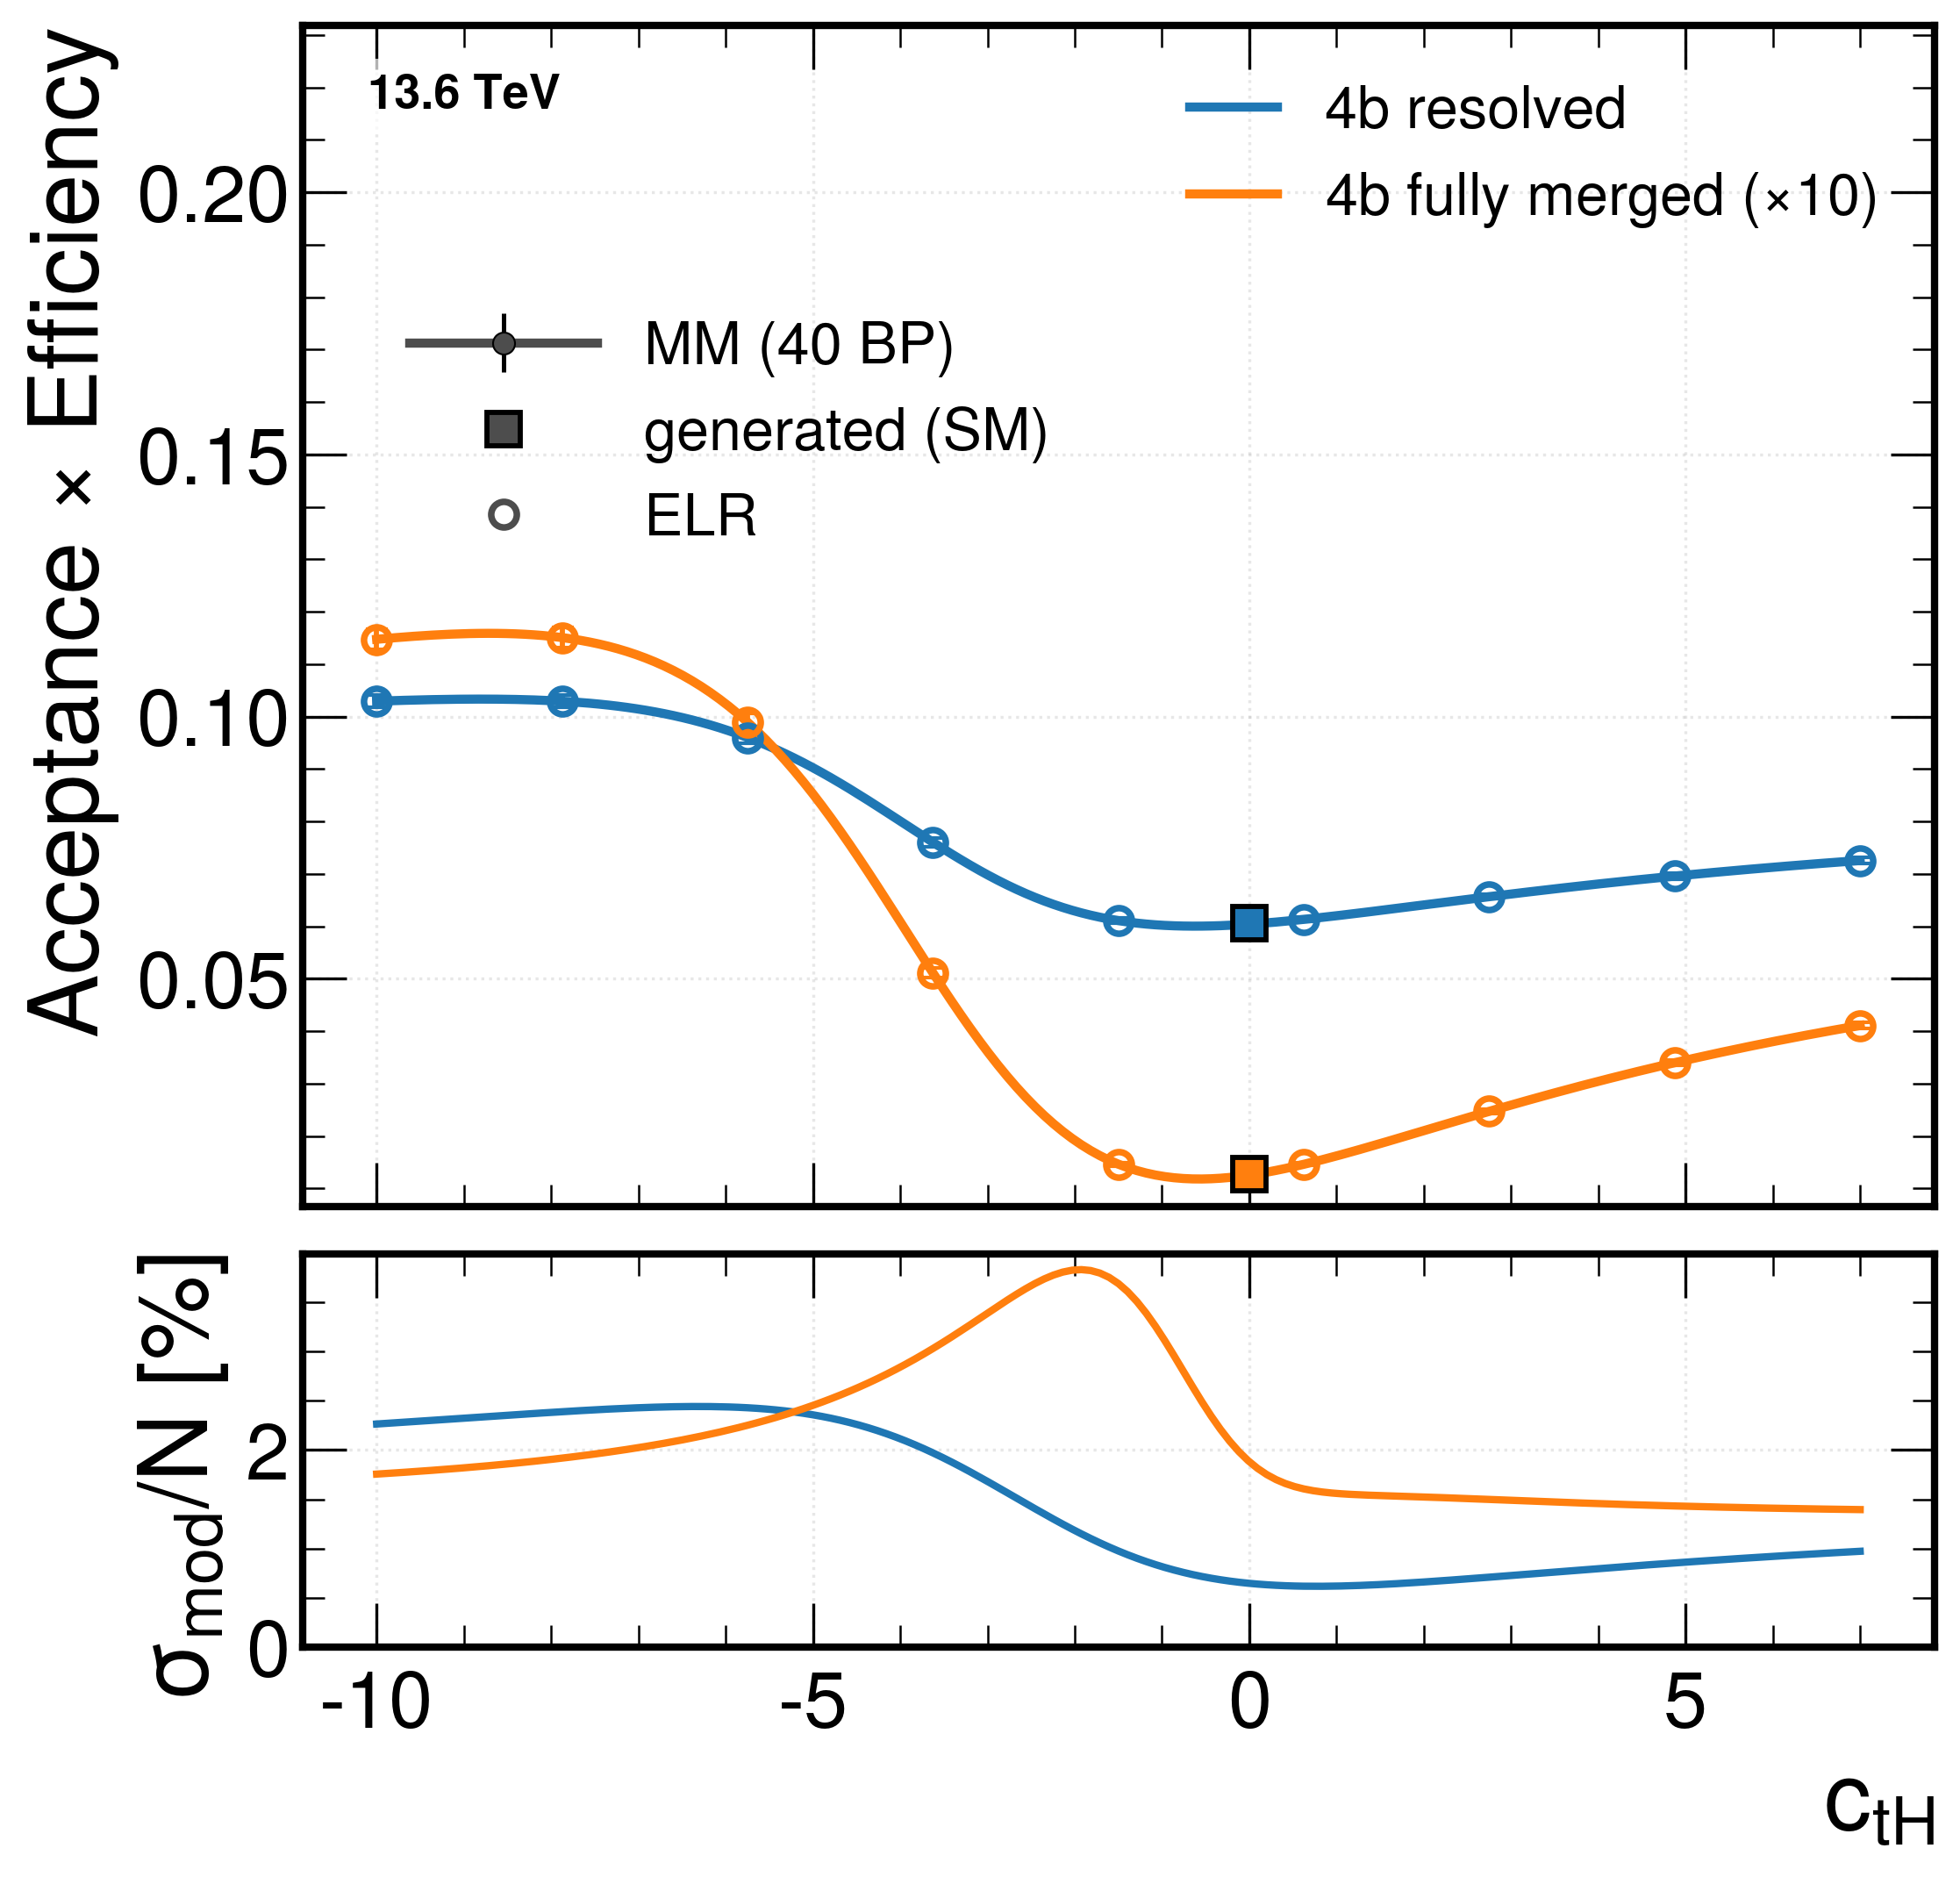
\includegraphics[width=0.32\textwidth]{figures/basis_optimization/eff4b_ctH.png} \\
    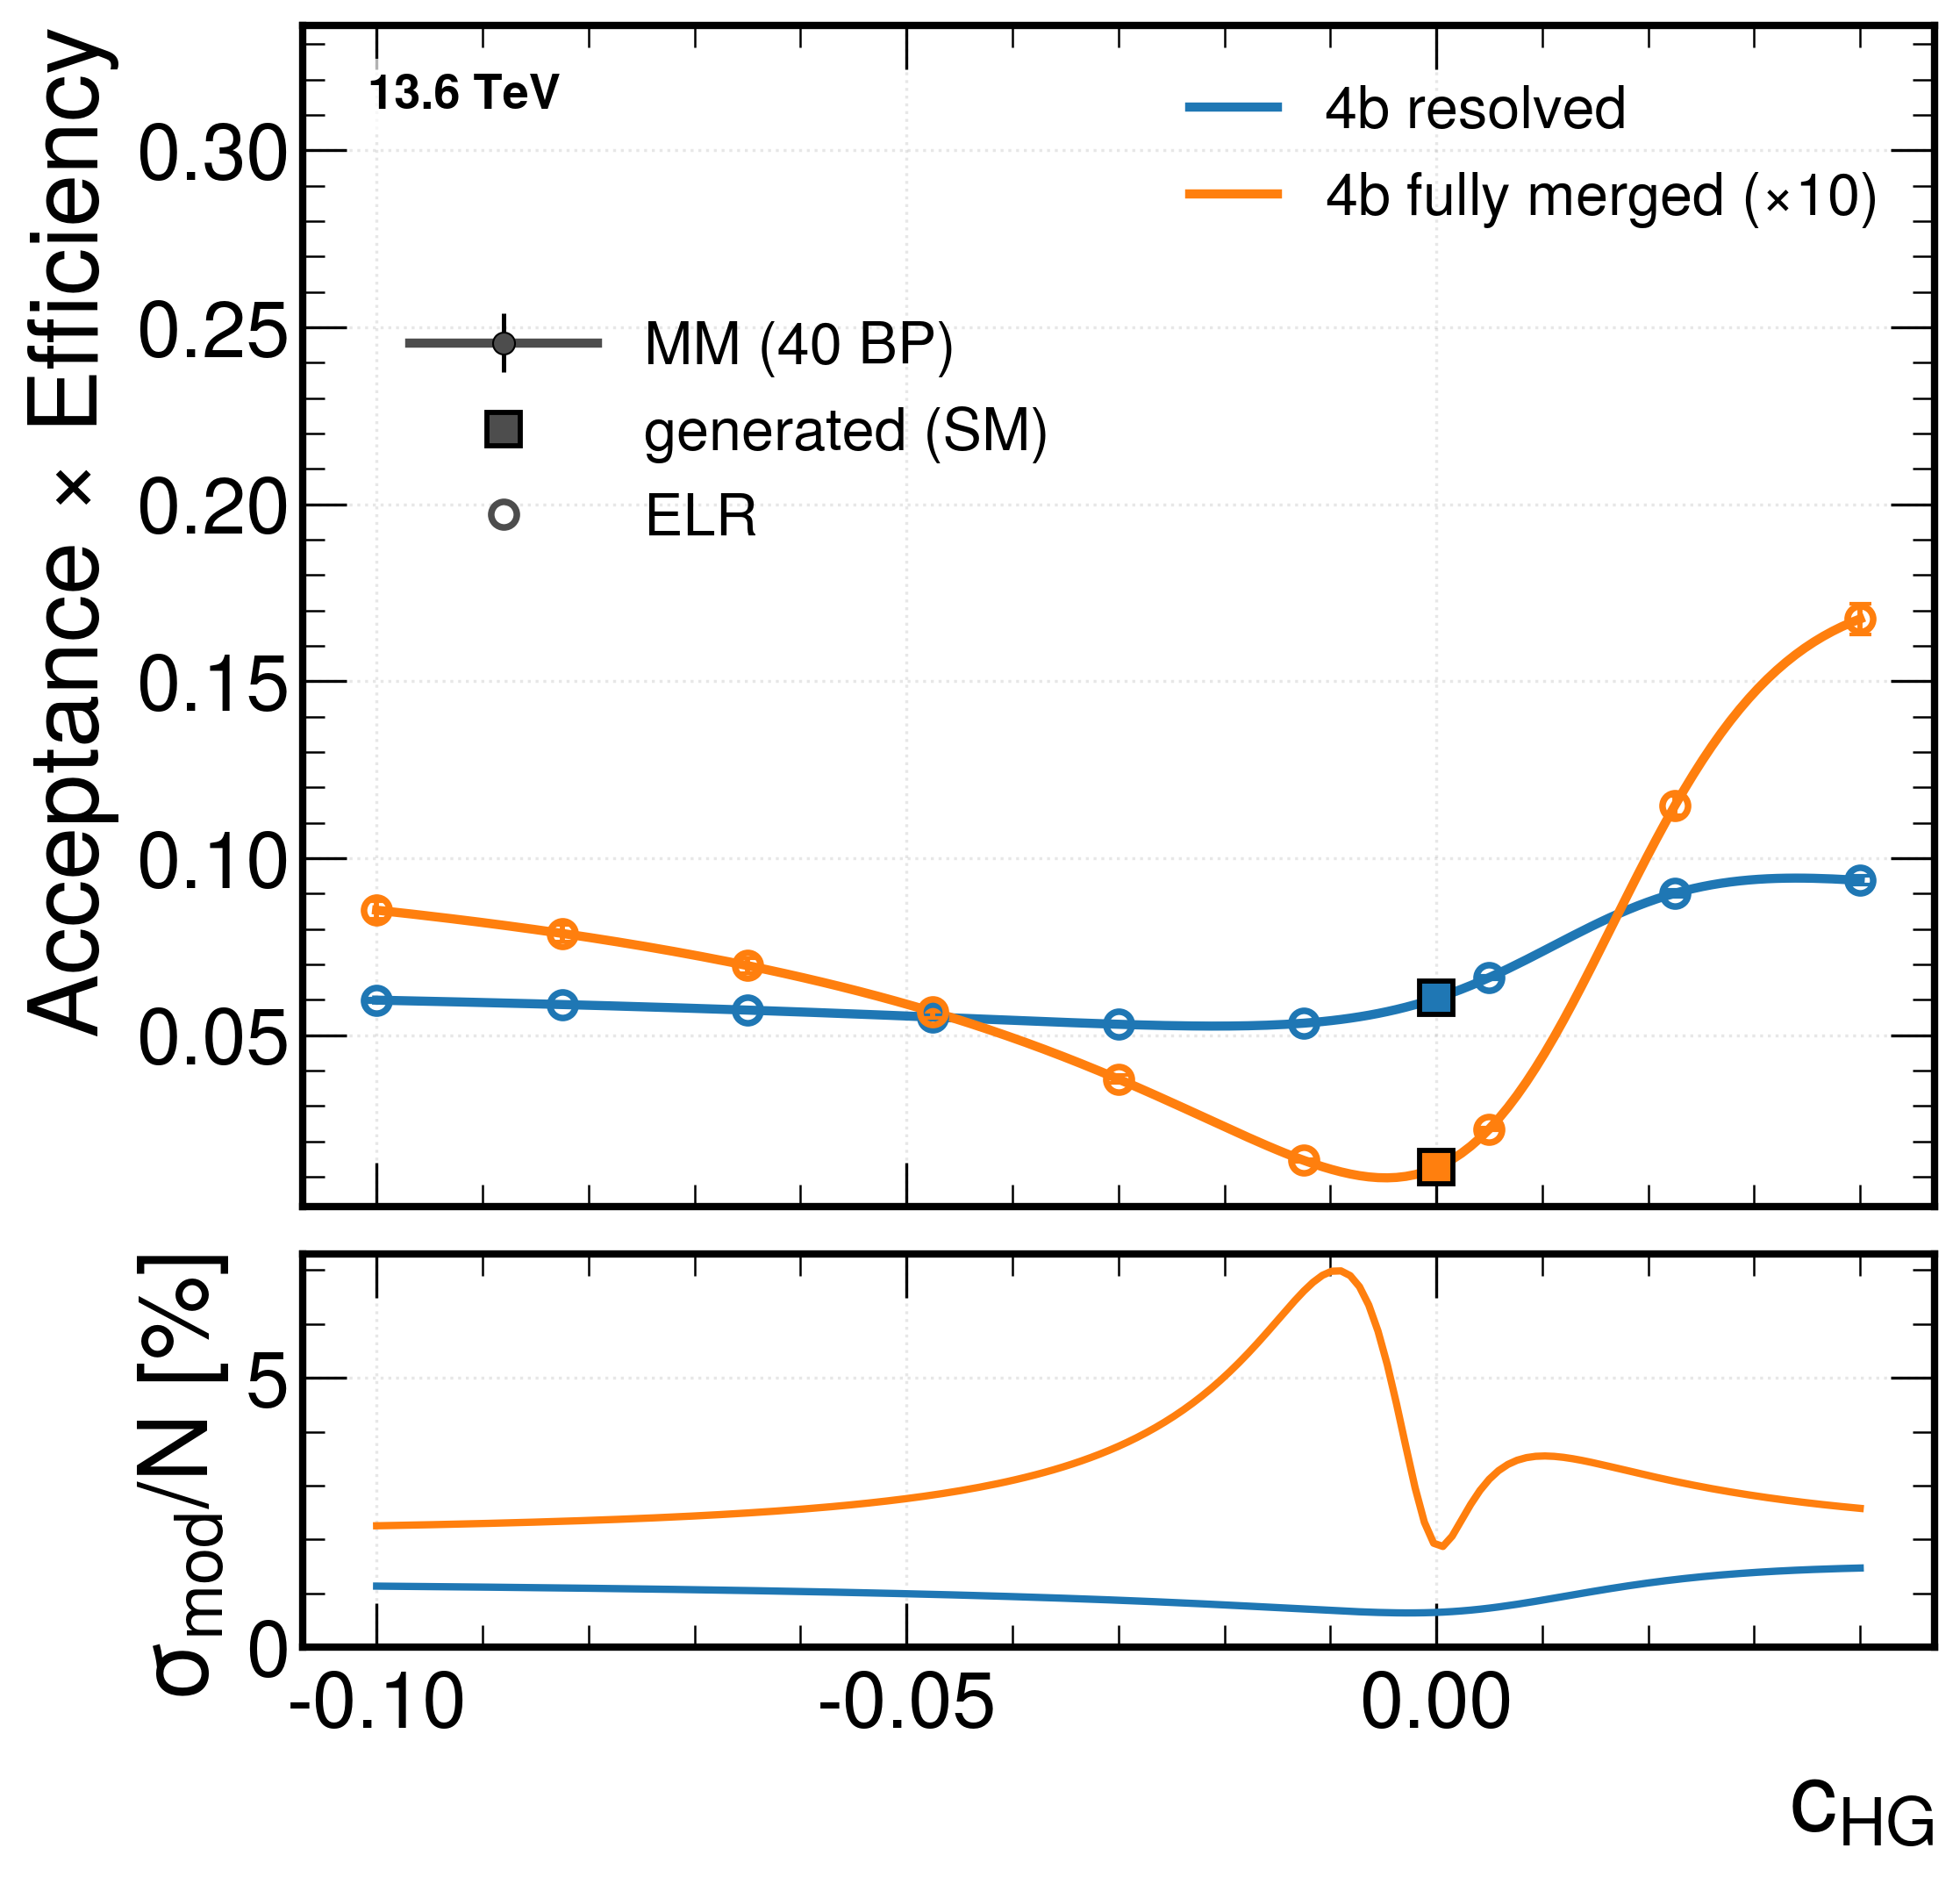
\includegraphics[width=0.32\textwidth]{figures/basis_optimization/eff4b_cHG.png} 
    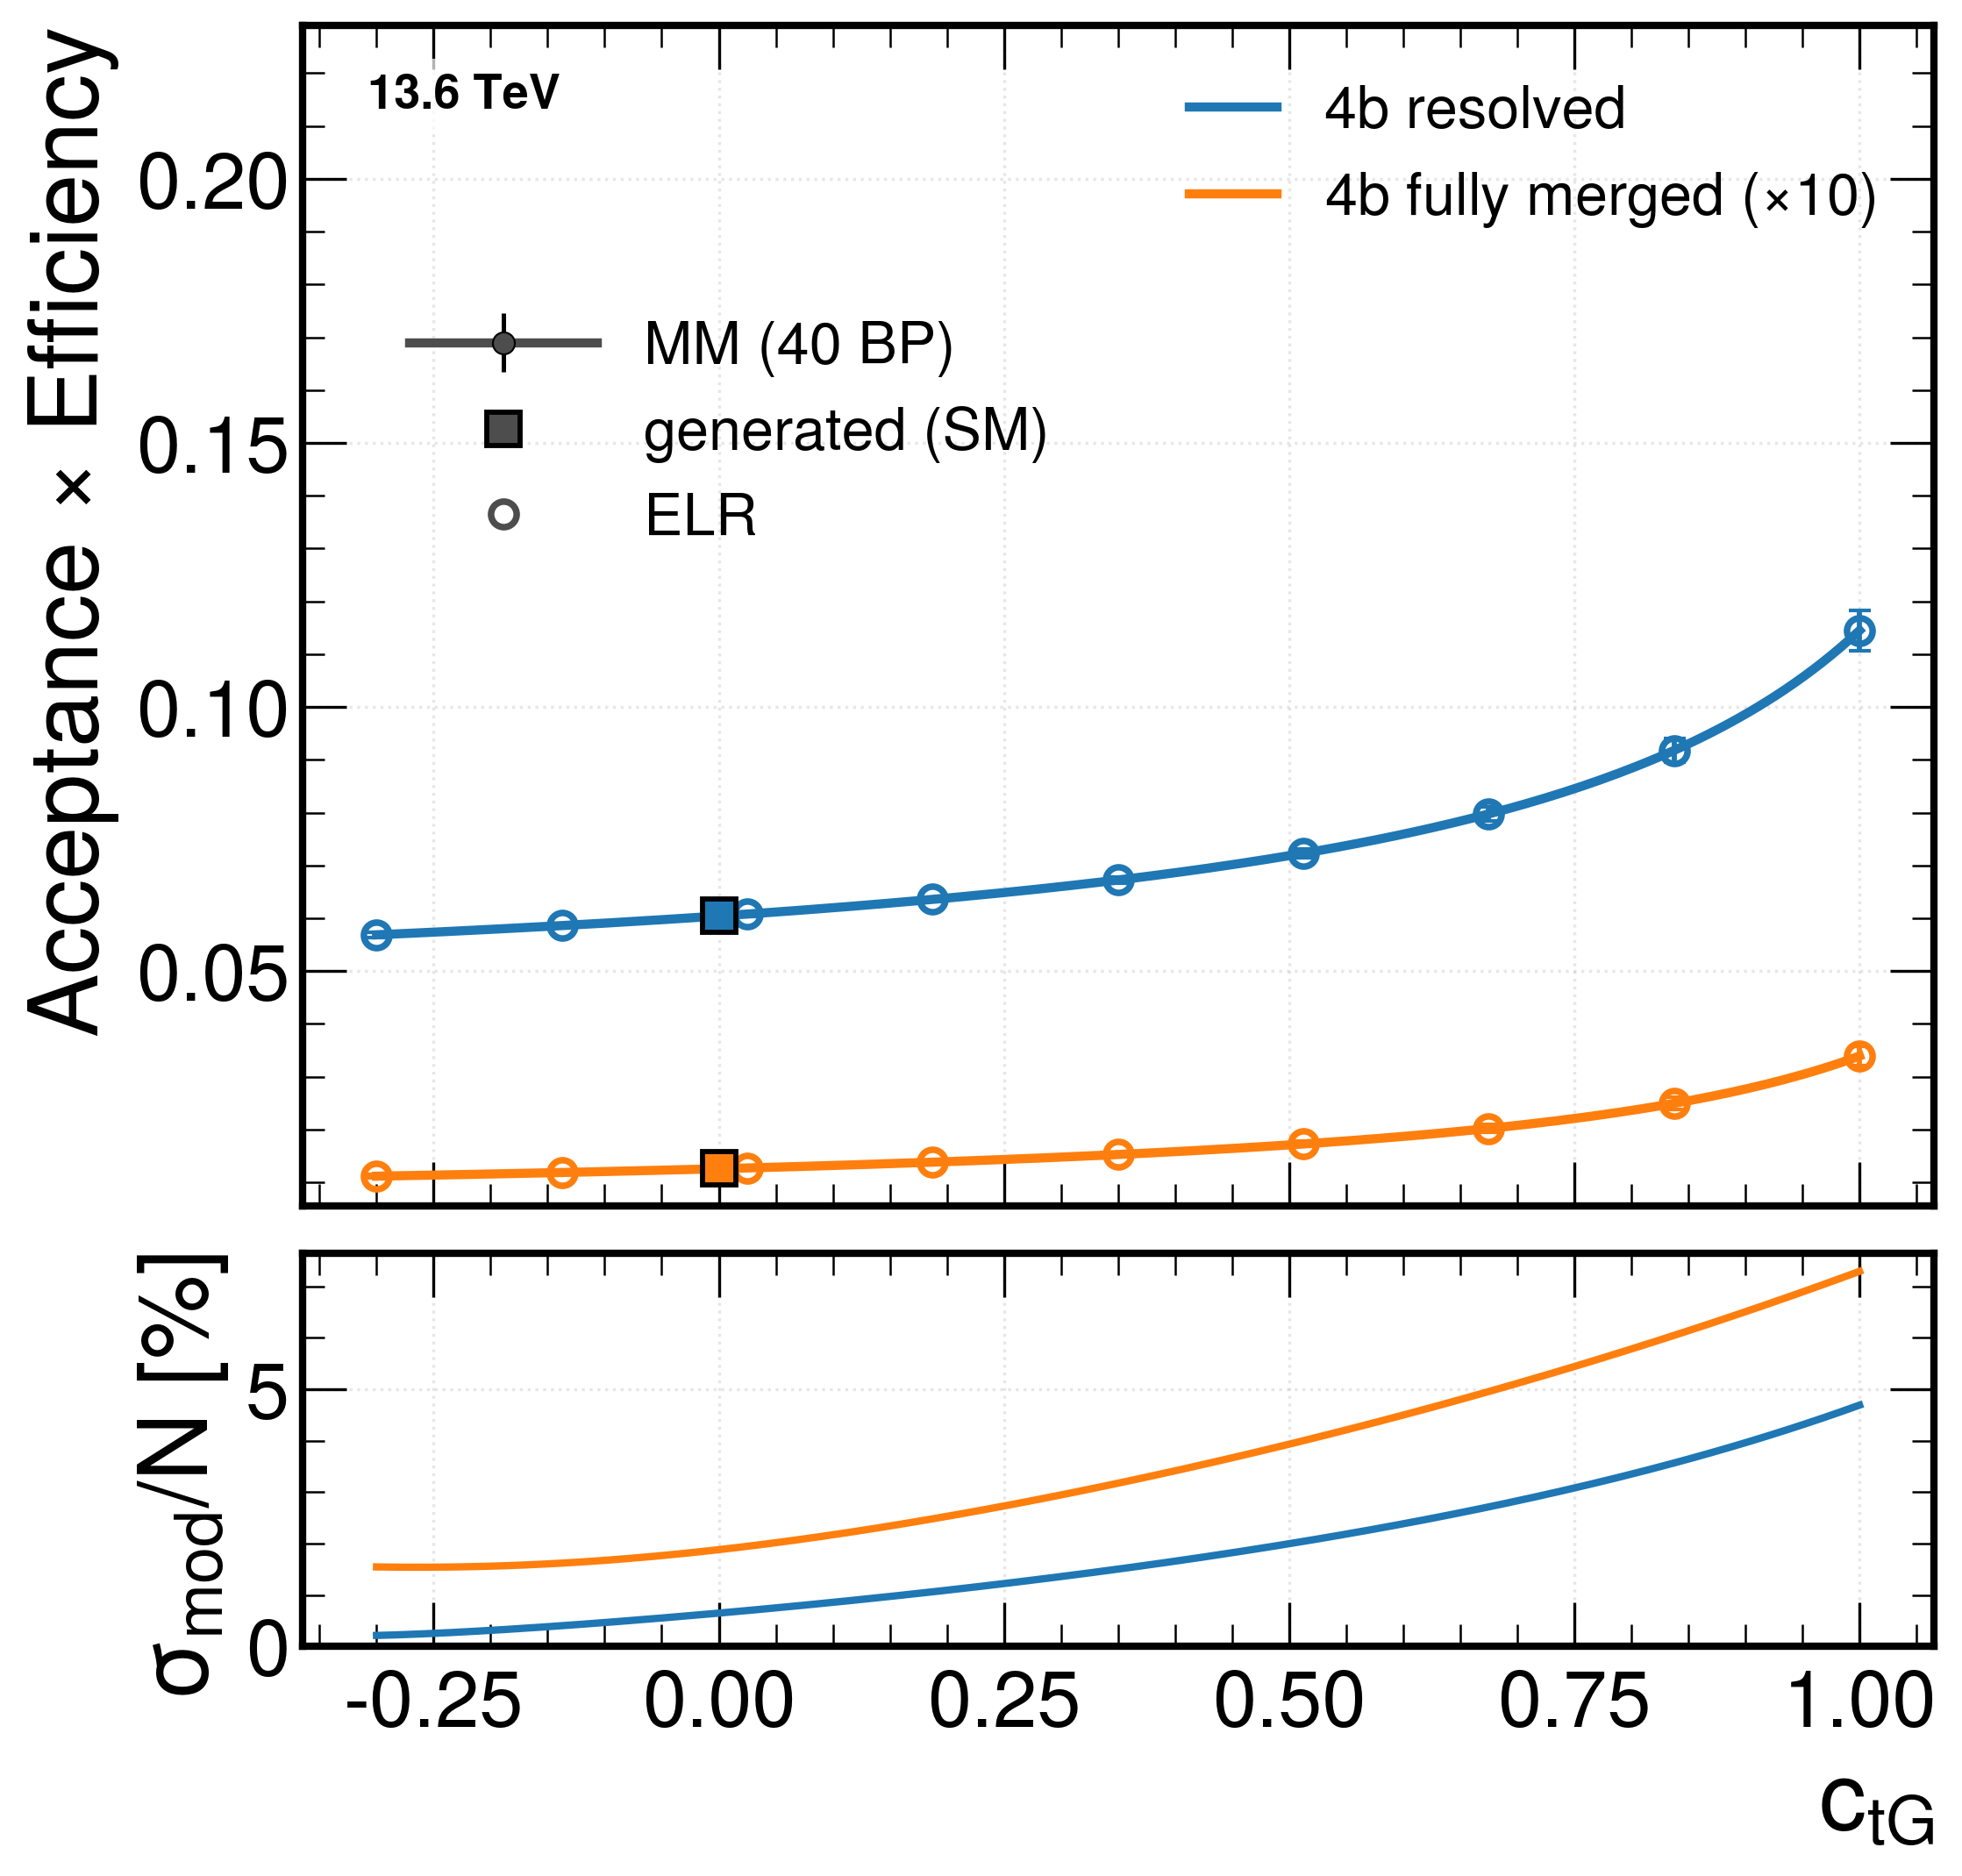
\includegraphics[width=0.32\textwidth]{figures/basis_optimization/eff4b_ctG.png}%
    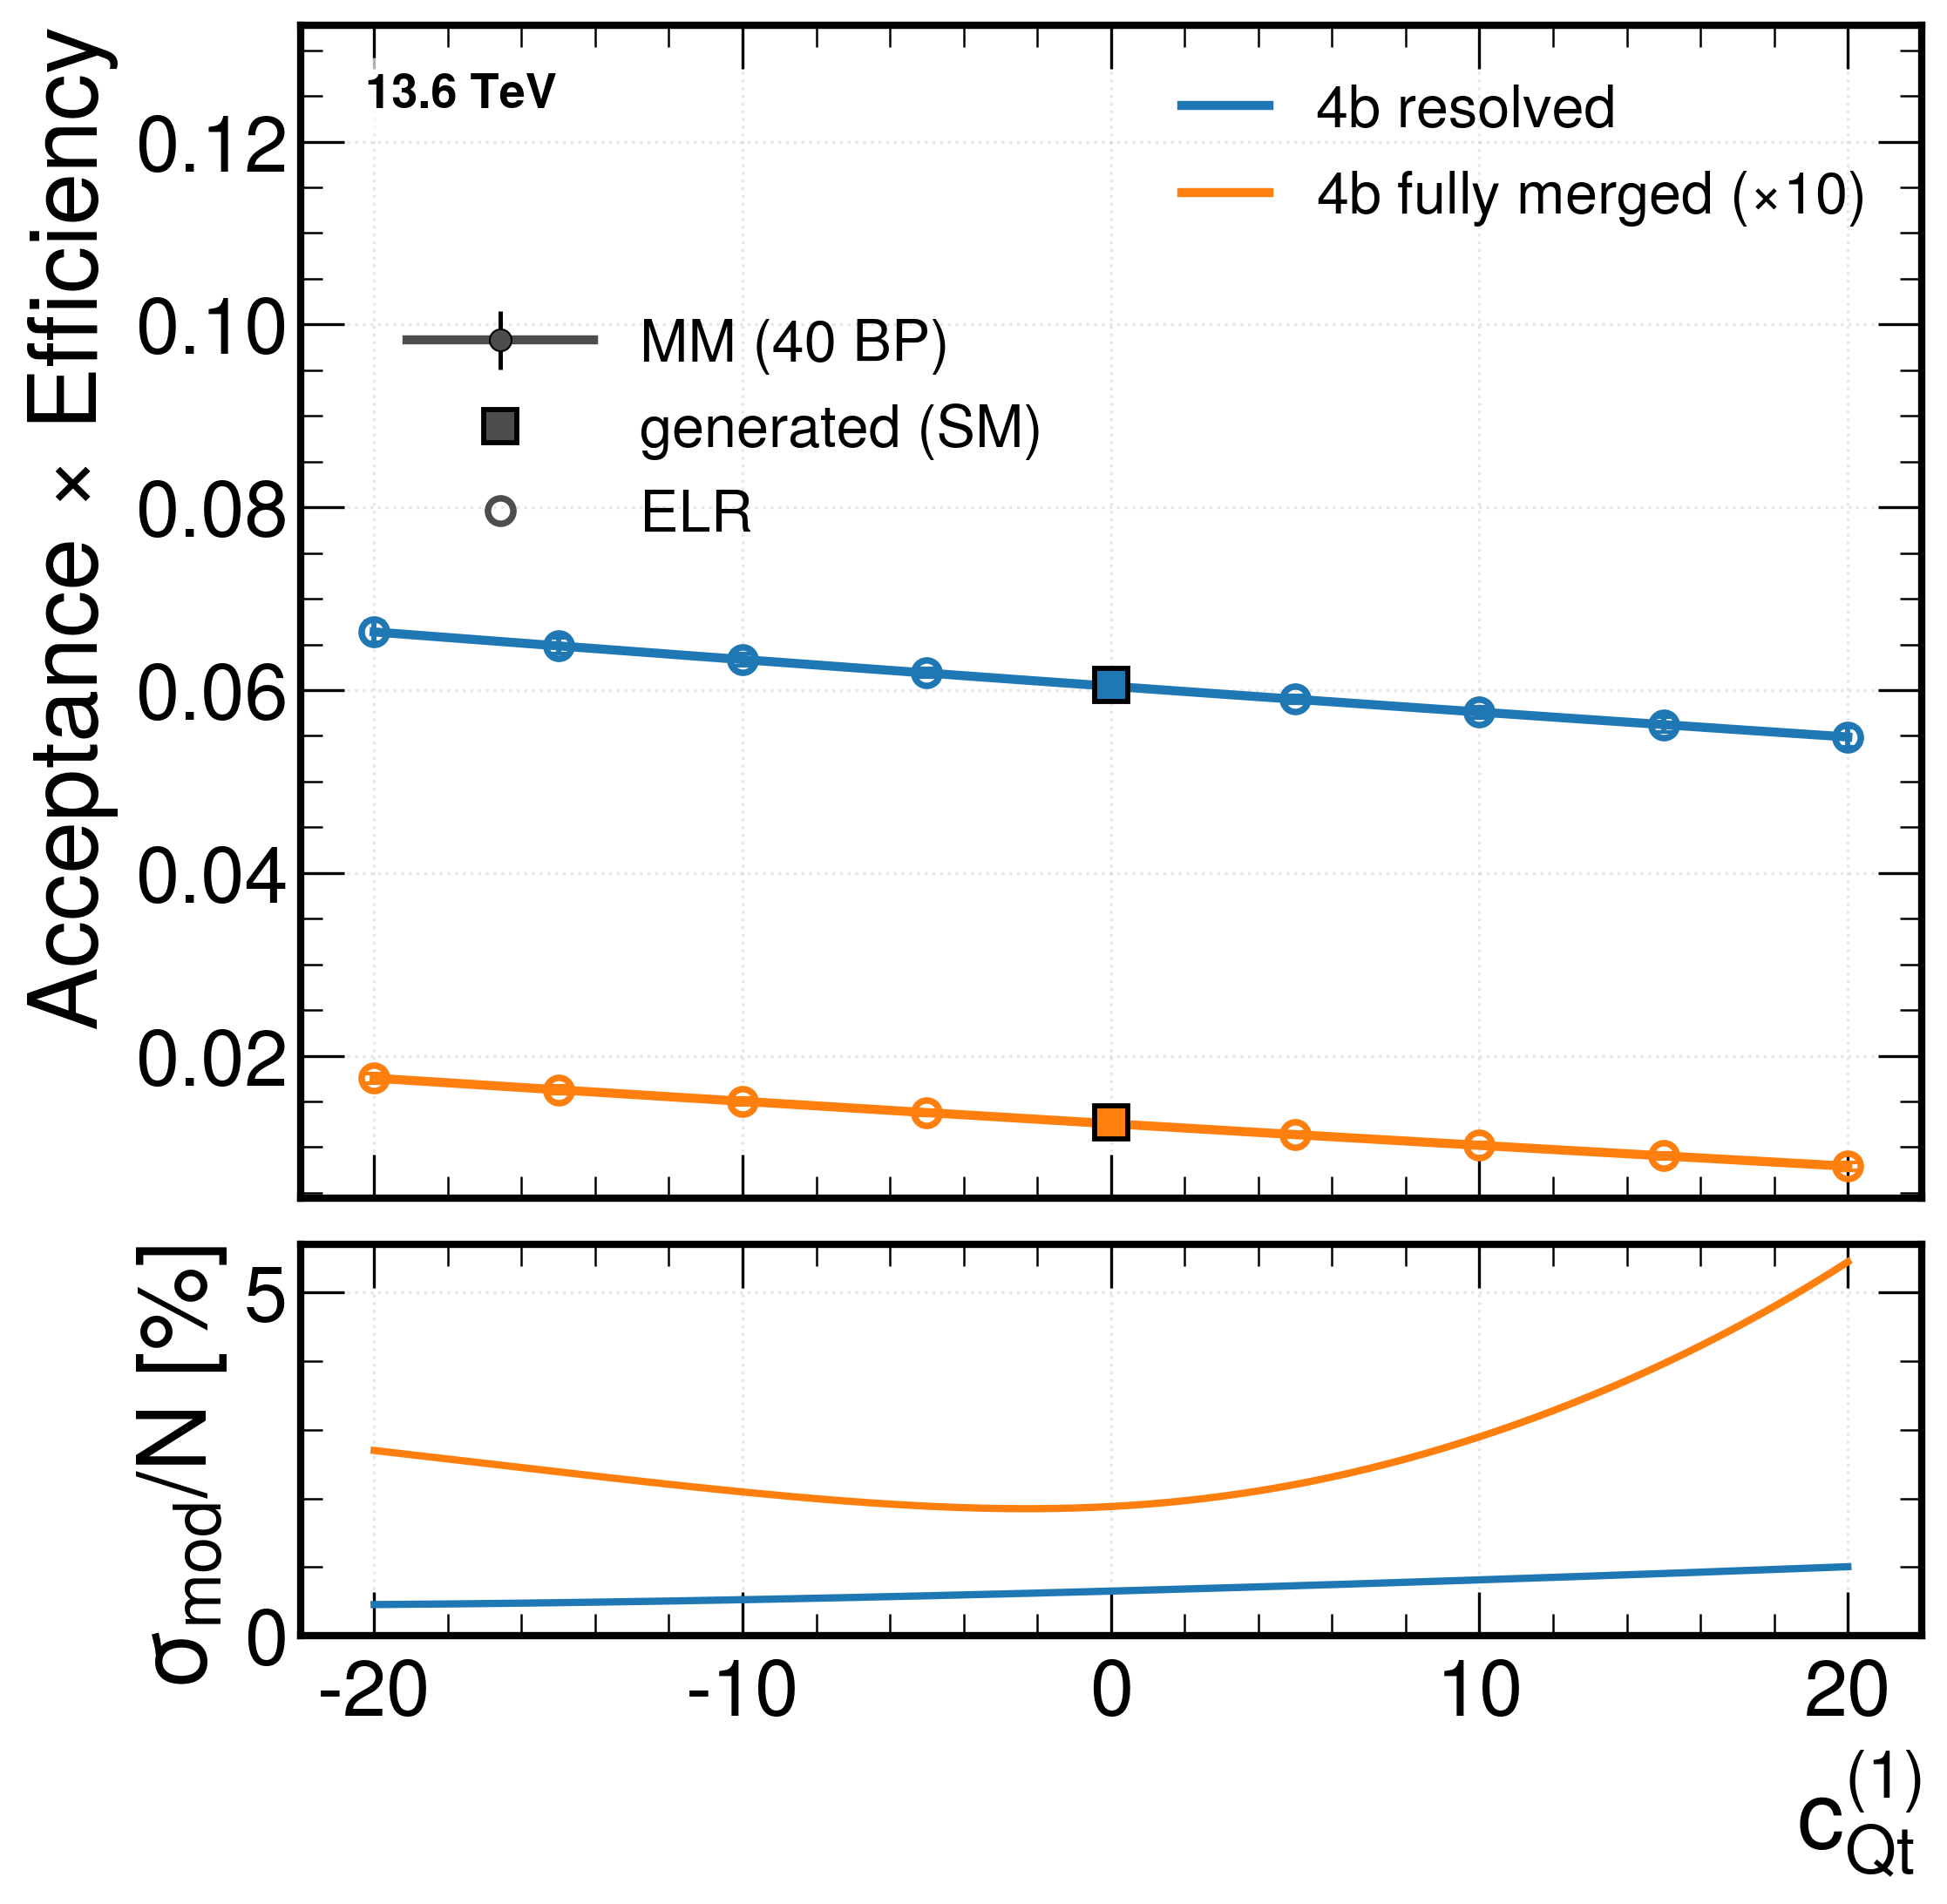
\includegraphics[width=0.32\textwidth]{figures/basis_optimization/eff4b_cQt1.png}
    \caption{Acceptance times efficiency against each Wilson coefficient, the other eight
held at zero, for the resolved and fully merged selections of Ref.~\cite{CMS:2026znu}. The merged curve is
multiplied by ten. Blue and yellow curves: the matrix method on the optimized basis, with bands combining
the statistical error of the templates and the uncertainty of the reweighting
coefficients. Open circles: the ELR applied directly on the corresponding points. Filled square: the directly generated $\kappa_\lambda=1$
sample (SM). Three coefficients are omitted: $c_{Q\PQt}^{(8)}$, $c_{QQ\PQt\PQt}$, and $c_{QQ}^{(8)}$, which have small response in both topologies.}
\label{fig:acc_4b}
\end{figure}
\begin{table}[htbp]
\centering
\begin{tabular}{l|cccc|ccccc}
\hline
 & \multicolumn{4}{c|}{leading} & \multicolumn{5}{c}{subleading} \\
 & $c_{\PH}$ & $c_{\PH\mathrm{kin}}$ & $c_{\PQt\PH}$ & $c_{\PH G}$ & $c_{\PQt G}$
 & $c_{Q\PQt}^{(1)}$ & $c_{Q\PQt}^{(8)}$ & $c_{QQ\PQt\PQt}$ & $c_{QQ}^{(8)}$ \\
\hline
4b resolved      & $0.79$ & $0.37$ & $0.96$ & $0.90$ & $1.03$ & $0.19$ & $0.17$ & $0.02$ & $0.00$ \\
4b merged  & $1.8$  & $3.6$  & $8.6$  & $13.2$ & $1.8$  & $0.78$ & $0.91$ & $0.09$ & $0.03$ \\
\hline
\end{tabular}
\caption{Relative spread over the scanned
range of each coefficient. This is obtained by computing the $(\max-\min)$ acceptance times efficiency divided by the value obtained at the SM value,
with the other eight coefficients held at zero. %The ranges are those of
%Table~\ref{tab:SMEFTcouplings}. $c_{\PQt G}$ is listed with the leading
%coefficients here because it behaves like them.}
}
\label{tab:acceptance_response}
\end{table}

%This setting also answers whether a separate, smaller basis is worth building for a
%linearly truncated interpretation. A ten-point basis for the interference-only prediction
%exists (Appendix~\ref{sec:appendix_linear}) and would cost ten simulated samples instead
%of forty. Applied to these two selections it does not work: four of its ten templates
%have a negative yield in the fully merged selection, and one, at $c_{\PQt\PH}=-10$ and
%$c_{\PH G}=-0.0567$, is negative in every region while its inclusive cross section stays
%positive, so it can enter a fit neither as a shape nor as a rate. The positivity imposed
%during the basis search acts on the inclusive total, and inclusive positivity does not
%survive a selection that favours the high-mass tail, which is where the truncated
%prediction is most negative. A basis search cannot repair this in advance because it does
%not know the selection.

%What fails is the saving, not the linear truncation. A linearly truncated prediction
%remains available from the forty-point basis: its templates are untruncated physical
%distributions, and the linear prediction is formed at evaluation by restricting the
%forty-coefficient solve to the ten linear monomials $A_0$--$A_4$ and $A_{15}$--$A_{19}$,
%which reproduces samples generated with the same truncation
%(Appendix~\ref{sec:appendix_linear}). No template is negative in that route, because no
%template is itself a truncated object; the truncated \emph{prediction} can still turn
%negative at large couplings, but that is the expansion leaving its validity window
%(Appendix~\ref{sec:appendix_trunc_validity}) rather than a defect of the basis. The cost
%is forty samples rather than ten, and the two bases are not interchangeable. An analysis
%restricting its coupling ranges may not meet the problem at all, since every negative
%point lies far from the SM. The measurements behind this are in
%Appendix~\ref{sec:appendix_linear_selection}.

\subsection{Which operators a selected phase space is sensitive to}
\label{sec:validation_subleading_role}

%Which Wilson coefficients change what an analysis measures is a property of the selection
%as much as of the operators, and the two selections of the $\HH\to\bbbar\bbbar$ release
%differ sharply enough to compare. The quantity is again the acceptance times efficiency,
%evaluated from the basis alone: it needs no simulation beyond the templates already made,
%and being a ratio it is insensitive to anything that scales the rate uniformly. An
%operator may change the cross section by a large factor and the acceptance not at all.




%Table~\ref{tab:acceptance_response} gives the response and Fig.~\ref{fig:acc_4b} shows
%it. Three things follow. The merged selection is more responsive than the resolved one by
%an order of magnitude for the coefficients it responds to at all: its acceptance is
%$0.11\%$ against $4.15\%$ at the SM, and it varies by a factor thirteen across the range
%of $c_{\PH G}$ where the resolved selection varies by a factor two. A selection keeping
%only the most boosted events is sensitive to the operators that populate the hard tail;
%the resolved selection, keeping most of the spectrum, averages over that structure.

%The ordering also changes between the two. In the resolved selection $c_{\PQt G}$ gives
%the largest response and $c_{\PH G}$ the third; in the merged one $c_{\PH G}$ dominates
%and $c_{\PQt G}$ falls to fifth. Which operator an analysis is most sensitive to is
%therefore not a property of the operator alone, and a statement of the form ``this
%analysis constrains $c_{\PH G}$ best'' is a statement about its selection.

%The four-fermion sector splits into two pairs. $c_{Q\PQt}^{(1)}$ and $c_{Q\PQt}^{(8)}$
%move the acceptance, $0.8$ to $0.9$ in the merged selection and comparable to $c_{\PH}$
%there, though below $0.2$ in the resolved one. $c_{QQ\PQt\PQt}$ and $c_{QQ}^{(8)}$ are
%consistent with no response, a spread of $0.00$ to $0.09$: neither selection separates
%the SM from the edge of the scanned range.

%Within each pair the two members are nearly degenerate, which bears on what a fit can
%separate. Normalizing each response to its SM value and comparing over the full range,
%$c_{QQ\PQt\PQt}$ and $c_{QQ}^{(8)}$ differ by $3\%$ and $c_{Q\PQt}^{(1)}$ and
%$c_{Q\PQt}^{(8)}$ by at most $20\%$, the difference confined to the merged selection
%above $c_{Q\PQt}\simeq5$; in the resolved selection they agree to $2\%$ everywhere. The
%two members of each pair are the colour-singlet and colour-octet forms of the same
%operator, so they enter through closely related topologies and differ only by colour
%factors. An analysis using the resolved selection alone cannot distinguish
%$c_{Q\PQt}^{(1)}$ from $c_{Q\PQt}^{(8)}$ by acceptance, however many samples it
%simulates. They do change the cross section, and Sec.~\ref{sec:validation_ladder} showed
%that the parameterization cannot describe the generated samples without them: their
%effect is close to a normalization, so an analysis measuring a rate will constrain them
%while one relying on the selection to separate them will not.

%No selection of this example therefore measures a four-fermion direction: two of them are
%flat and the other two are degenerate with each other. Carrying them in the parameterization buys
%something else. They are needed to describe the generated samples
%wherever they are switched on, which is what Sec.~\ref{sec:validation_ladder} measures,
%so a five-coefficient description fitted to such a region would absorb their effect into
%the coefficients it does have; and they are the coefficients through which the
%renormalization-group running reaches the Higgs operators at all
%(Sec.~\ref{sec:rge}).

A scan through one coefficient holds the others at zero, which hides whatever two of them
do jointly. Fig.~\ref{fig:planes} shows the acceptance
over three planes: the two coefficients the merged selection responds to most strongly,
the pair in which the cross section has its cancellation, and the strongest leading
coefficient against the strongest subleading one. No plane is drawn with $c_{QQ\PQt\PQt}$
or $c_{QQ}^{(8)}$, along which nothing happens, and none with $c_{\PQt G}$ against
$c_{Q\PQt}^{(1)}$, which is vertical banding: the acceptance depends on the first and not
on the second, as the one-dimensional scans already say. These are the only
two-dimensional figures in this report, and they are affordable because the acceptance is
evaluated from the basis: a plane costs model evaluations, not simulation.

Two things about reading the figure. The merged panels are multiplied by ten and each row then
shares one colour scale, so that colours may be compared across a row; without the
scaling the two panels would be coloured on ranges a factor forty apart. And the crosses
are the forty basis points projected on the plane --- their two coordinates in it, the
other seven ignored --- so a cross marks where the basis constrains the surface read
along those axes, not that a template was simulated at that point. Most of the forty have
their two non-zero couplings elsewhere and project onto the axes of the plane.

\begin{figure}[p]
    \centering
    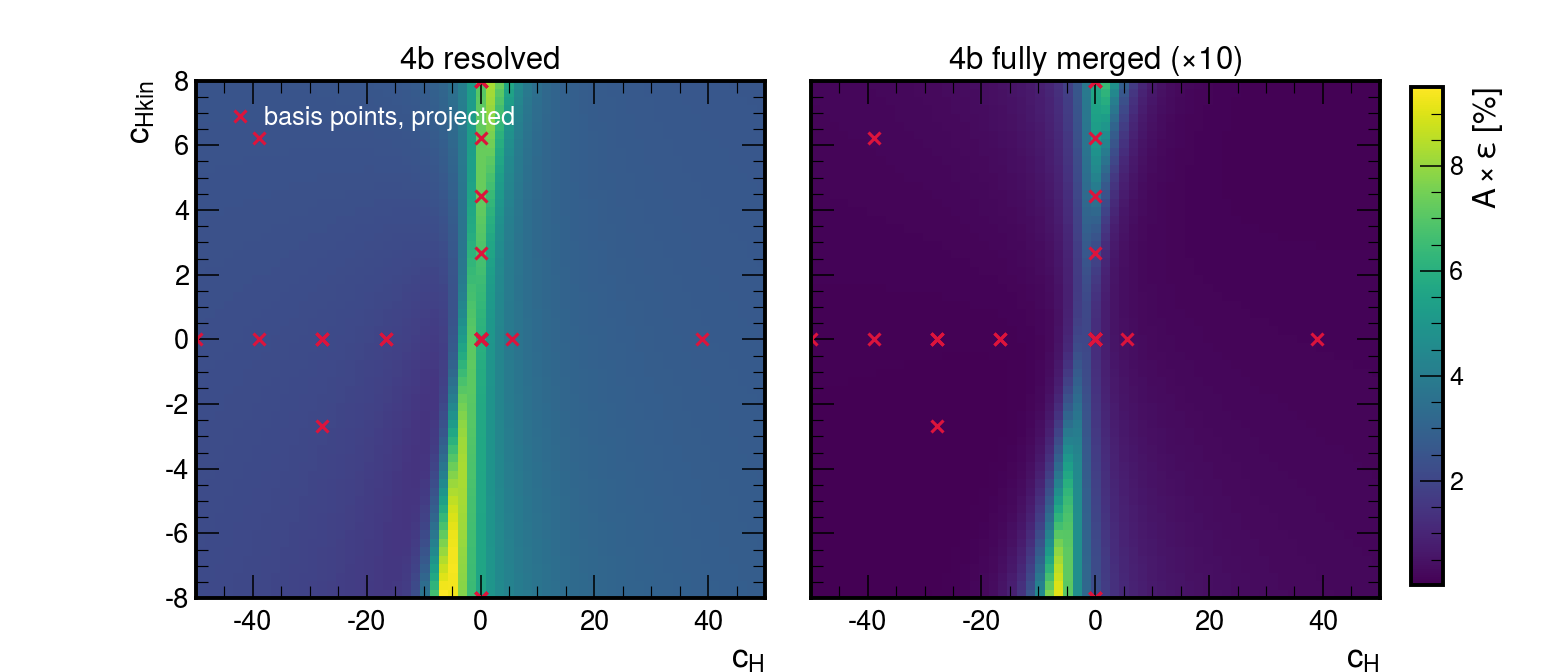
\includegraphics[width=0.88\textwidth]
        {figures/basis_optimization/plane_cH_cHkin.png}\\[4pt]
    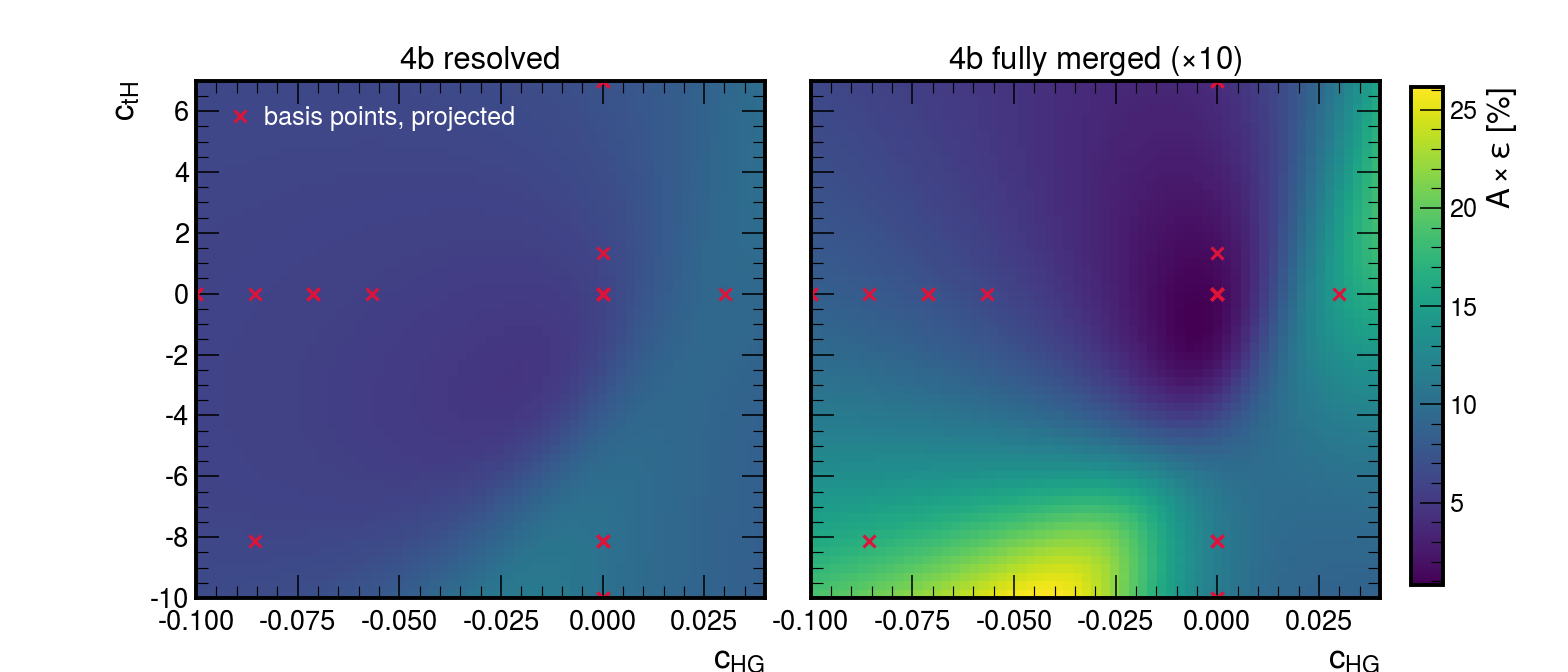
\includegraphics[width=0.88\textwidth]
        {figures/basis_optimization/plane_cHG_ctH.png}\\[4pt]
    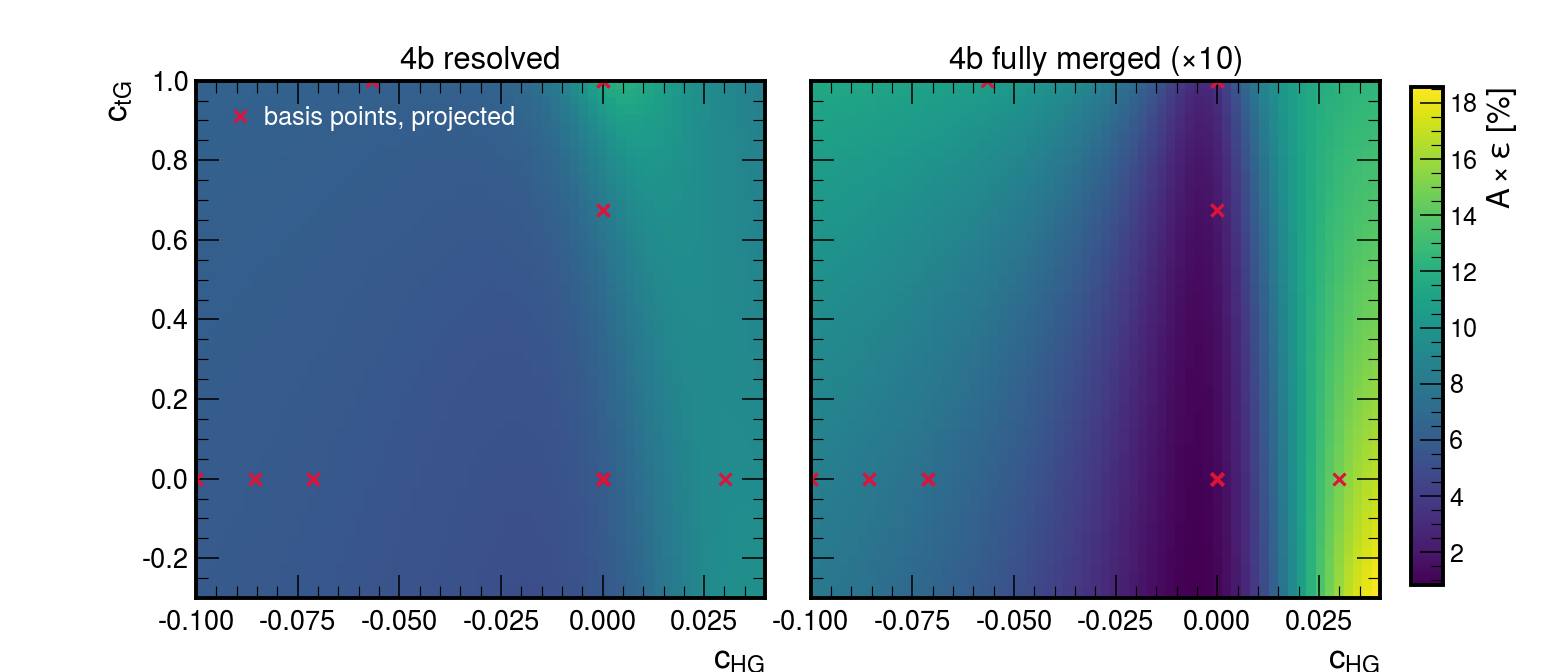
\includegraphics[width=0.88\textwidth]
        {figures/basis_optimization/plane_cHG_ctG.png}
    \caption{Acceptance times efficiency over three coupling planes, the other seven
    coefficients at zero, for the resolved (left) and fully merged (right) selections of
    Ref.~\cite{CMS:2026znu}. From top to bottom:
    $c_\PH\mbox{--}c_{\PH\mathrm{kin}}$, $c_{\PH G}\mbox{--}c_{\PQt\PH}$ and
    $c_{\PH G}\mbox{--}c_{\PQt G}$. Each merged panel is scaled by ten and shares the
    colour range of the resolved one in its row. Crosses are the basis points of
    Table~\ref{tab:smeft_basis_9d} projected on the plane.}
    \label{fig:planes}
\end{figure}

\subsection{The interpolation uncertainty an analysis would quote}
\label{sec:validation_realistic_band}

An analysis that adopts the basis of this report derives nothing about the effective field
theory in order to obtain its interpolation uncertainty. The statistical error of the forty
templates propagates with the same weights the prediction uses,
Eq.~\eqref{eq:sigmainterp}, evaluated independently in every bin; the derivation and its
calibration against the residual observed are in Sec.~\ref{sec:uncertainties}. The weights $w_i(\mathbf{c})$ are a
property of the basis alone: they follow from the parameterization and the forty points,
they are the same in every bin, and they are independent of the selection applied and of
the quantity being histogrammed. They are published once, with the basis. The $\sigma_i$
are the statistical errors of the basis templates as the analysis itself has them, after
its own trigger, reconstruction and selection, in its own fit variable, with its own
binning.

The two selections of Ref.~\cite{CMS:2026znu} turn that statement into a measurement. One
set of weights is applied to the template errors of the resolved selection and to those
of the fully merged one, and nothing else is changed: the parameterization, the basis
points and the weights are the ones used everywhere above, and the only input that
differs is the set of $\sigma_i$. The scans hold the other eight coefficients at zero and
cover the full generated range of the one varied, as in Fig.~\ref{fig:acc_4b}.

The two bands differ throughout. Tab.~\ref{tab:unc_components} collects them for the six
coefficients of Fig.~\ref{fig:acc_4b}. In the resolved selection the band is between
$0.14\%$ and $0.28\%$ of the yield at the median of a scan and at most $2.06\%$; in the
fully merged selection the medians are between $0.99\%$ and $2.76\%$ and the largest
value is $6.85\%$, along $c_{\PH G}$. At the SM the band is $0.17\%$ of the resolved
yield and $1.26\%$ of the merged one. The weights entering the two numbers are identical,
so the difference is entirely in the $\sigma_i$: the merged templates hold far fewer
events. This is the same mechanism as the bin-by-bin behaviour of
Sec.~\ref{sec:uncertainties}, with a selection in place of a bin.

Figs.~\ref{fig:unc_realistic_cH} and \ref{fig:unc_realistic_cHkin} of
Appendix~\ref{sec:appendix_unc_per_selection} show the yield and the band along $c_\PH$
and $c_{\PH\mathrm{kin}}$; the remaining four are in
App.~\ref{sec:appendix_performance}. The two selections are drawn on one logarithmic axis
rather than side by side: the quantity being compared is the lower panel, which is a
ratio and is unaffected by the factor of some forty between the two acceptances. The two
bands differ in size and peak at different coupling values, because the cancellation
between the contributions to the rate sits at a different coupling value once the
selection has reshaped them. Neither feature could be obtained from the other selection's
band by rescaling it. A band measured in one category is therefore not an estimate of the
band in another, and the number an analysis needs is obtained by applying the published
weights to the errors of its own templates, in its own categories, which is the
calculation performed here with two sets of templates and one set of weights.

These two bands and the inclusive ones of Tab.~\ref{tab:unc_bands} share only the
weights: the inclusive $\sigma_i$ are estimated from the event count and the
negative-weight fraction of the generated samples (Sec.~\ref{sec:uncertainties}), so the
two sets of numbers are not to be compared point by point.

The bands here are computed from Eq.~\eqref{eq:sigmainterp}, which treats the template
errors as independent. These templates are reweightings of one set of events and are
therefore correlated, and the independent form overstates the band away from a basis
point --- by up to a factor of nine integrated over \mHH and about thirty in a single
bin. The exact form, Eq.~\eqref{eq:sigmaMMcov}, needs the covariance of the templates
and is what an analysis should use; the numbers below are quoted in the independent form
because that is the one that can be evaluated from a delivered yield table
(Sec.~\ref{sec:uncertainties}). The shaded bands contain the Monte Carlo statistical
error of the templates and nothing else. The uncertainty of the reweighting coefficients
the templates were made with is a separate term, and the larger of the two at almost
every point. Measured on the same templates it is a median of $1.48\%$ and at most
$4.69\%$ in the resolved selection, and a median of $1.91\%$ and at most $15.17\%$ in the
merged one. Propagated along a one-dimensional scan, the up and down variations of those
coefficients largely cancel in the weighted sum, so a band built from them is visible
only where the weights load onto basis points whose reweighting error is large, which
among these six scans is the $c_{\PH\mathrm{kin}}$ axis. The figures therefore understate
the total uncertainty of the templates. An analysis carrying both terms adds them in
quadrature in each bin; the double counting discussed in Sec.~\ref{sec:uncertainties}
does not arise when it does so, because its templates are built from its own events while
the reweighting coefficients come from the generated grid.

Obtaining either band requires no step of the effective field theory to be repeated and
no correspondence between an analysis's selection and the ones used here. An analysis
binning in $\pt^{\PH}$, in a classifier output, or in several categories at once obtains
a band in each of them; an analysis whose selection removes most of the threshold region
obtains a band that reflects that, without the selection having been anticipated when the
basis was built. The uncertainty is propagated differentially, through quantities the
analysis already has. A closure
uncertainty quoted as a single number per scan point, as would follow from comparing
total rates, could not be transported in this way: it would describe the phase space it
was measured in, and an analysis selecting a different one would have no means of
correcting it.

\subsection{Reducing the fit cost when few coefficients are free}
\label{sec:slice_models}

Most results are likelihood scans in one or two Wilson coefficients, with the rest held
at their SM values or a few of them profiled. The workspace, however, carries all forty
templates of the basis and evaluates all forty terms of Eq.~\eqref{eq:smeftpara_reorg}
in every bin, including the terms that depend only on coefficients the fit never moves.
Those terms are constants, and once they are constant the weight $w_i(c)$ of many basis
templates is exactly zero everywhere in the scan. A template whose weight is zero
contributes nothing to any prediction the fit will make, and can be left out of the
workspace.

One free coefficient leaves three of the forty terms and two leave six, and the number of
templates with a non-vanishing weight follows: between five and fifteen on a single axis,
about ten on a plane, and all forty once every coefficient moves. The count depends on
the direction and not only on the number of free coefficients --- the
$c_{\PH\mathrm{kin}}$ axis keeps six templates and the $c_{\PH G}$ axis fifteen --- and
it follows from the basis in one evaluation for any other scan. The coefficients that
have to be kept are those the fit scans, profiles, or holds at a value other than the SM
one.

Nothing new has to be simulated. The smaller model is the same card with templates
removed, so it can be built for any scan from the basis already in hand.

What is saved is the size of the statistical model. The expected yield of a bin is
$\sum_i w_i(c) N_{ij}$, so the work per bin is the number of templates times the number
of terms, and the two shrink together; Table~\ref{tab:slices} gives both, for the full
basis and for two scans, with the cost of one prediction and of one scan point. The
scan-point column is measured on a complete analysis model --- of order twenty
categories, parametric shapes with discrete profiling, the full set of systematic
uncertainties, and the $80$ templates of the nine-coefficient basis at two
centre-of-mass energies --- in which one point of a nine-coefficient scan takes about
half an hour against the tens of seconds an analysis with a handful of signal templates
is used to. Those are order-of-magnitude figures from one model and will differ between
analyses.

A global fit floats all nine coefficients, so it carries every template and saves
nothing. Three precautions apply to it, as general practice rather than as responses to
an observed failure. The minimiser is run with tight settings, since what a loose
tolerance saves is small next to a scan point that has not converged. Several starting
points are tried, because the cross section is quadratic in the coefficients and the
likelihood need not be unimodal: in a realistic nine-coefficient scan the $c_{\PQt G}$
direction shows a second minimum near $c_{\PQt G}=1$. And a coefficient the selection
does not respond to is fixed rather than floated, with the choice stated, so that no flat
direction enters the fit. On the measurement of
Sec.~\ref{sec:validation_subleading_role} those are $c_{QQ\PQt\PQt}$ and
$c_{QQ}^{(8)}$, whose acceptance varies by less than $0.1$ over their full range in
either $4\PQb$ selection: they move the rate and leave the shape untouched, so a fit that
floats them is fitting a direction its selection cannot see.
\textcolor{red}{Whether that survives at a collider reaching much higher \mHH, where the
four-top operators grow fastest, is a question for the $100$~TeV study
(Sec.~\ref{sec:energy_beyond}).}

For a channel as light as the \HHbbbb example used here the difference changes little in
practice: the model has few categories, and a scan that takes half an hour per point is
still affordable. The reduction is worth making where the model is heavy --- many
categories, several decay channels combined into one fit, and scans that have to be
repeated for each variation --- which is where the cost of carrying forty templates
through every bin becomes the limiting one.

The numerical results are unchanged, as they have to be: the templates that are dropped
carry a weight of zero, and the agreements measured on the \HHbbbb example are in
Table~\ref{tab:slices}, down to $10^{-5}$ in $-2\Delta\ln L$ with up to three
coefficients profiled and $2\times10^{-3}$ with up to seven. The Monte Carlo statistical
uncertainty of the morphed prediction is unchanged for a separate reason: the templates
are reweightings of the same simulated events, and their morphing reproduces the direct
reweighting to the target point in any basis (Sec.~\ref{sec:uncertainties}). Measured
along the $c_{\PH\mathrm{kin}}$ axis with the full covariance of the templates, the two
models give the same $\sigma_{\text{MM}}$ to the three digits quoted, from $0.173\%$ of
the yield at the SM point to $0.240\%$ at $c_{\PH\mathrm{kin}}=8$; integrated over \mHH
they agree to $0.1\%$ and per bin to within $4\%$. The interpolation uncertainty belongs
to the input samples rather than to the basis.

\begin{table}[htbp]
\centering
\begin{tabular}{lcccccc}
\hline
free & terms & templates & products & direct & one scan & agreement with \\
coefficients & kept & kept & per bin & evaluation & point & the full model \\
\hline
all nine (full basis)             & $40$ & $40$ & $1600$ & $9\,\mu$s   & $\sim30$~min & reference \\
$c_{\PH}$, $c_{\PH\mathrm{kin}}$  & $6$  & $10$ & $60$   & ---         & ---          & $5\times10^{-7}$ \\
$c_{\PH\mathrm{kin}}$             & $3$  & $6$  & $18$   & $0.2\,\mu$s & $\sim6$~min  & $<10^{-9}$ \\
\hline
\end{tabular}
\caption{Cost and agreement of the reduced model. ``Products per bin'' is the number of
templates times the number of terms kept. The direct evaluation is the prediction of the
\HHbbbb example outside any fitting framework; the scan point is one point of a
likelihood scan in a complete analysis model and is an order of magnitude only.
Agreement is the largest difference in $-2\Delta\ln L$ between the reduced and the full
model over the scans tested.}
\label{tab:slices}
\end{table}

A smaller model again can be built by giving the scan its own basis points --- three on
one axis, six on a plane, as many as the terms it keeps --- instead of keeping whichever
of the forty templates survive there. Those points are reweighted templates the card
does not already contain, so this is worthwhile only when the same scan is repeated.

Nothing in the construction is specific to the SMEFT parameterization: it needs only
that the prediction is a polynomial and that the morphing weights are polynomials in the
same terms. The same arguments apply to any physics case built with the matrix method,
HEFT among them.

